\section*{\begin{tabular*}{\linewidth}{@{}l @{\extracolsep{\fill}} r@{}}
Nr.~16 & MUN~87/2-1-1 \\
\end{tabular*} 
}

\textsf{\textbf{Munda (Likwala-aux-Herbes; Fpl.~304)}}

\vspace{1em}

\noindent\begin{tabular}{@{}rl@{}}
\textbf{Feldarbeit:} & \textbf{19.08.--30.08.1987 (F. Nikulka)} \\ 
\textbf{Abb.:} & \textbf{\ref{fig:MUN87.2-1-1-5_Foto}--\ref{fig:MUN87.2-1-1_Sequenz_Skizze}} \\ 
\textbf{Tab.:} & \textbf{\ref{tab:MUN87-2-1-1_Funde}--\ref{tab:MUN87-211_14C-Daten}}\\
\textbf{Taf.:} & \textbf{91.1--8} \\ 
\textbf{Lit.:} & \textbf{--} \\ 
\end{tabular} 

\paragraph{Grabung und Befunde}\hspace{-.5em}|\hspace{.5em}%
Nordwestlich der Grabung MUN~87/1 und direkt vor dem Eingang eines Hauses wurde eine leicht ovale Verfärbung beobachtet, die von einem fast geschlossenen Ring aus rotgebranntem Lehm umgeben war. Neben Fragmenten von Gefäßen und Stücken gebrannten Lehms lagen auch Schlacken an der Oberfläche. Der Befund wies einen Durchmesser von 0,95--1,0\,m auf und der Profilschnitt wurde so angelegt, dass auch die direkt nördlich gelegene Grube MUN~87/2-1-3 (Kat.-Nr.~17) ausgegraben werden konnte.\footnote{Der zweite Teil beziehungsweise die westliche Hälfte des Befundes MUN~87/2-1-1 wurde aus Zeitmangel nicht ausgegraben.} Die Grabung erfasste einen aus drei stratigrafisch klar differenzierbaren Bereichen bestehenden Befund (Abb.~\ref{fig:MUN87.2-1-1_Planum+Profil_Zeichnung}).

Die obere Verfüllung C reichte bis etwa 0,85\,m unter die rezente Oberfläche und war stark mit Schlacken und Keramikgefäßen durchsetzt. Im zweiten Abtrag, nur etwa 0,2\,m unter der Oberfläche, fand sich in der Mitte der Grube und unterhalb eines stark zerscherbten Keramikgefäßes ein flaches Eisenobjekt (Abb.~\ref{fig:MUN87.2-1-1_Planum+Profil_Zeichnung}, \ref{fig:MUN87.2-1-1-2_Eisengeld_Foto}).\footnote{Das Objekt lag nahezu horizontal in Nord–Süd-Richtung orientiert, mit der Spitze nach Süden weisend.} Um die Situation um das auf der Seite liegende Gefäß 3 (Taf.~91.1) und den Charakter der die obere Verfüllung (C) umschließenden, rotgebrannten Lehmwanne (B) näher zu untersuchen, wurde ein Ost--West ausgerichtetes Querprofil angelegt (Abb.~\ref{fig:MUN87-211-4_F87-02-36}--C).\footnote{Direkt an die stark mit Schlacke durchsetzte Verfüllung schließt sich eine 0,5--1,0\,cm starke, schwarz-reduzierend gebrannte Zone (Abb.~\ref{fig:MUN87-211-4_F87-02-31}: 1) an, die in die eigentliche Lehmwanne übergeht (Abb.~\ref{fig:MUN87-211-4_F87-02-31}: 2). Diese besteht aus extrem hart gebrannten, blass-gelben Lehmbrocken, die zwischen 3--5\,$\times$\,4--8\,cm groß sind. Die Wanne ist in den anstehenden Lehm eingetieft, der mehrere Zentimeter rot verziegelt ist (Abb.~\ref{fig:MUN87-211-4_F87-02-31}: 3). Zwischen den blass-gelben bis gelb-rötlichen gebrannten Lehmbatzen fanden sich stellenweise ebenfalls Schlacken. Im nördlichen Bereich besteht die Wandung der Grube lediglich aus rot verziegeltem Lehm. Im südlichen Bereich sind sowohl der anstehende rot verziegelte Lehm als auch härter gebrannte rotgefärbte Lehmbatzen (2) vorhanden, die auf eine zusätzliche Auskleidung der Grube mit Lehm hindeuten. Im Bereich des Gefäßes 3 verjüngt sich der rot verziegelte Lehm deutlich. Direkt hinter dem Gefäß ist er nur noch zirka 1\,cm stark. Beim Abtragen des Querprofils (Abb.~\ref{fig:MUN87-211-4_F87-02-36}--C) wurde eine deutliche Konzentration von Schlacken gefunden. Bis knapp unterhalb des dritten Abtrages sind zwischen den gebrannten Lehmbatzen auch noch viel ungebrannte Lehmstücke aufgetreten, was nahe legt, dass die Brocken wohl erst nach dem Brand mit der Verfüllung in die Grube gelangt sind.} Das Gefäß ist direkt in die Ofenwandung (B) hinein gesetzt worden. Unterhalb von Gefäß 3 und mehr zur Grubenmitte hin fand sich ein vollständiges, ebenfalls auf seiner Seite liegendes Gefäß (Abb.~\ref{fig:MUN87-211-5}--B: 2; Taf.~91.5). Nach der Bergung der Gefäße wurde deutlich, dass die Schlacke nicht mit der Keramik verschmolzen war.\footnote{Alle Gefäße und Gefäßfragmente waren aber von einem Substrat umgeben, das sehr viel Schlacke sowie rötlich-braunen Lehm, durchsetzt mit Partikeln rot-gebrannten Lehms, enthielt.} Die Wandung der Lehmwanne (B) ist im nördlichen Bereich bis etwa 0,35--0,40\,m unter der Oberfläche flachschräg (Abb.~\ref{fig:MUN87-211_Oben}, \ref{fig:MUN87.2-1-1_Planum+Profil_Zeichnung}). Unterhalb ist sie hingegen vertikal bis senkrecht.

\begin{figure*}[p]
	\centering
	\begin{subfigure}{\columnwidth}
		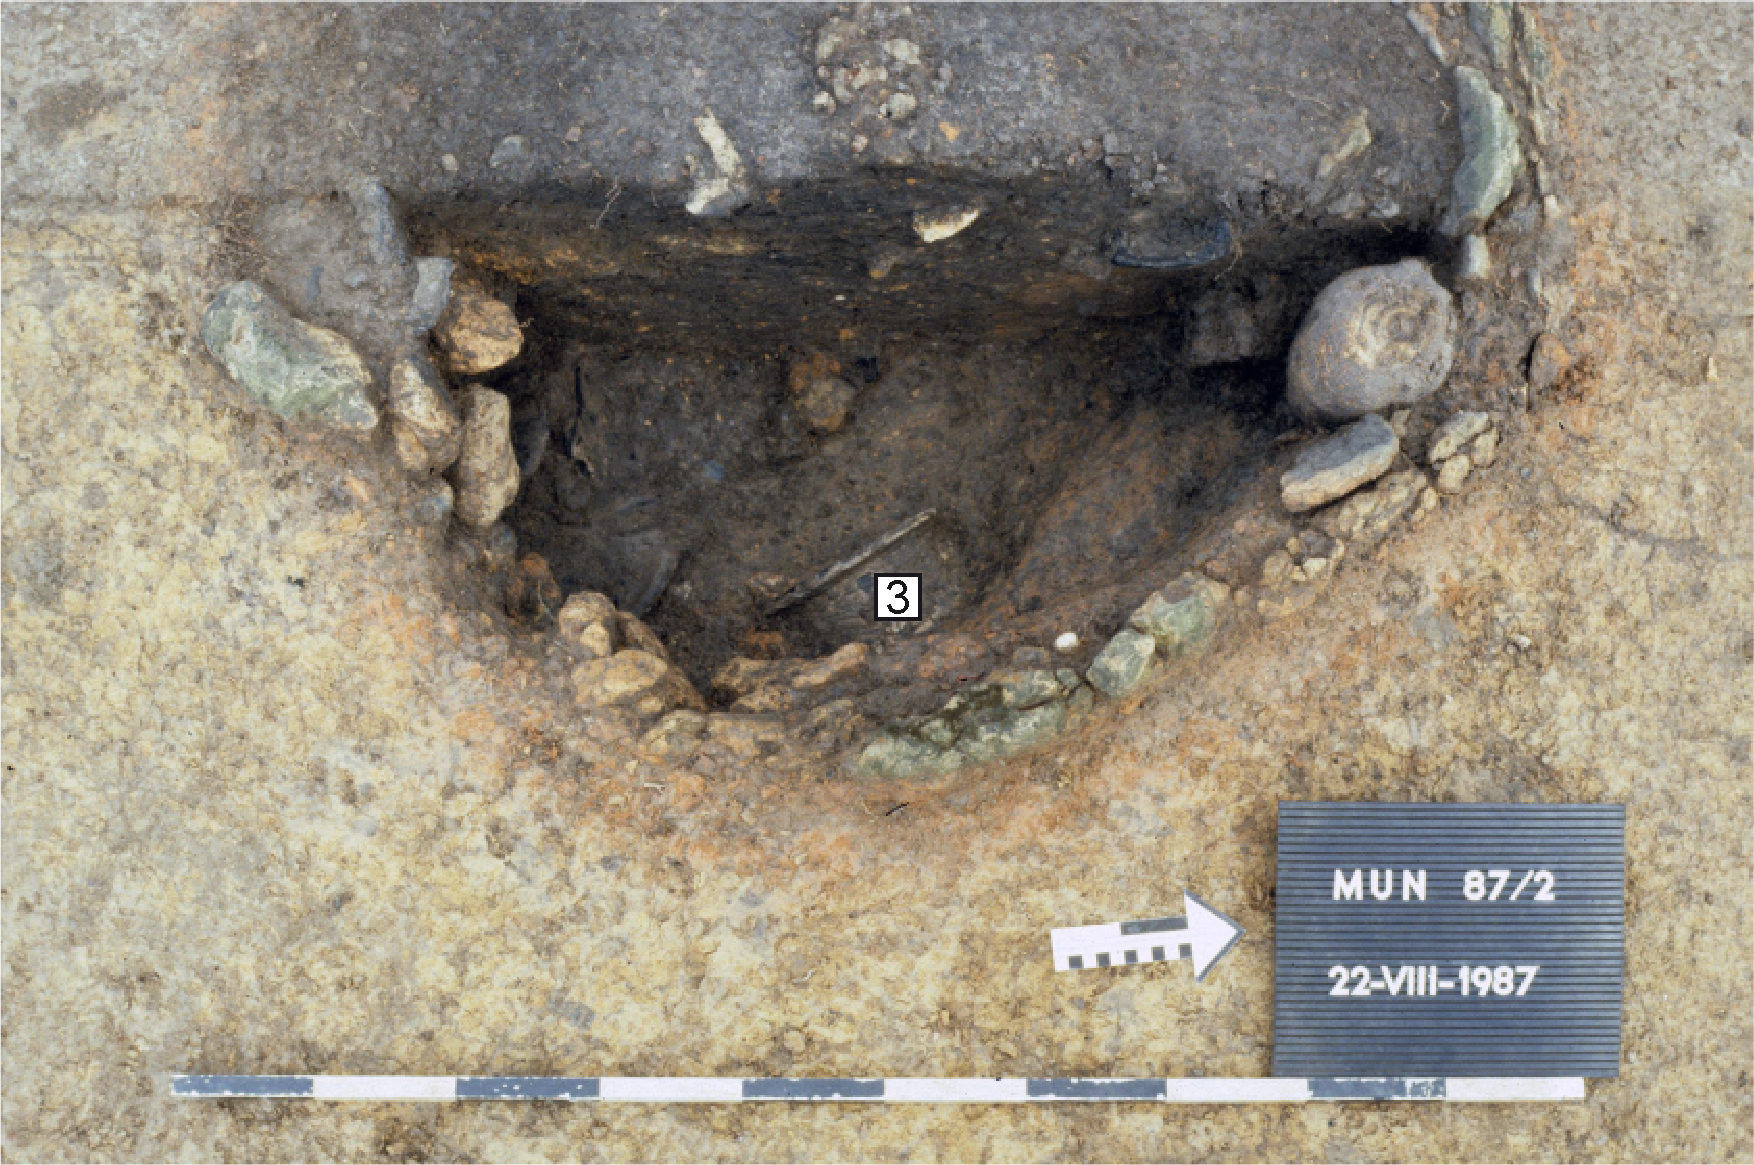
\includegraphics[width = \textwidth]{fig/MUN87-211-3_F87-02-27.pdf}
		\caption{Abtrag 4 (Foto: F. Nikulka, 1987).}
		\label{fig:MUN87-211-3_F87-02-27}
	\end{subfigure}\hfill
	\begin{subfigure}{\columnwidth}
		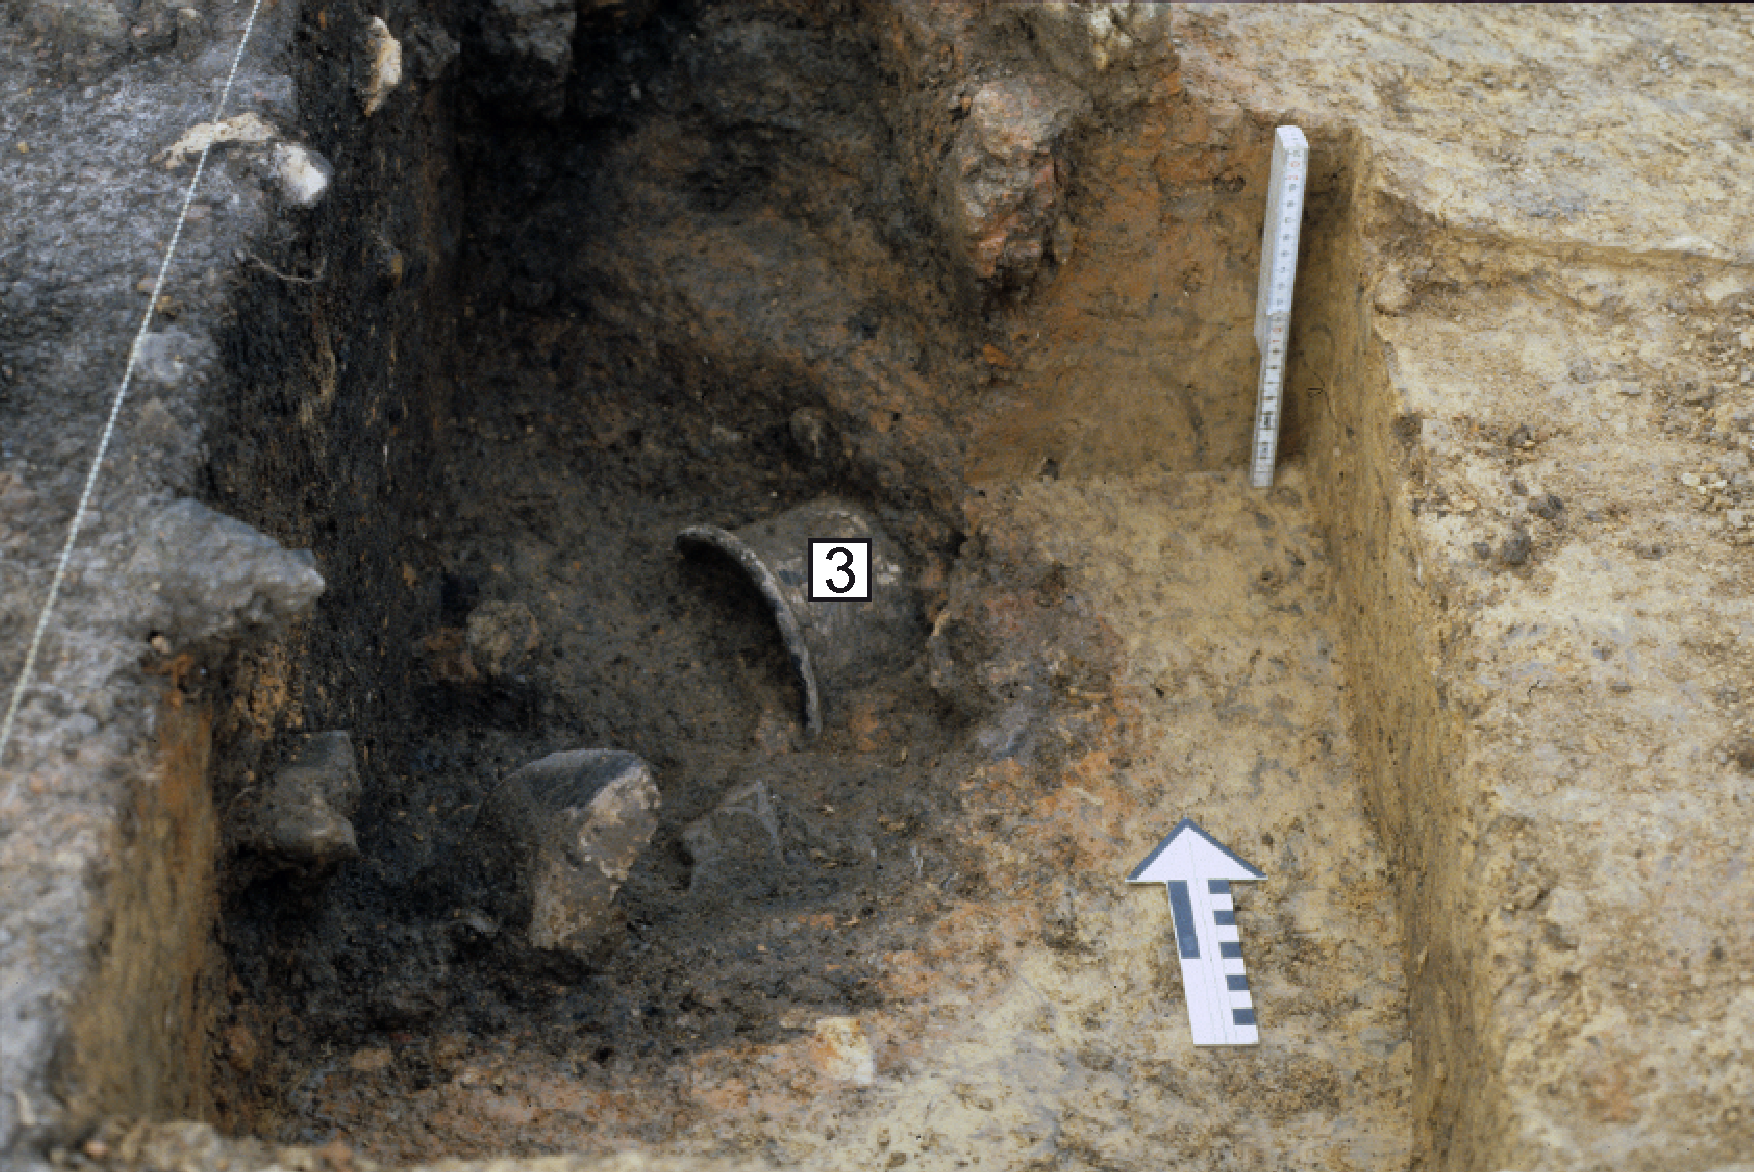
\includegraphics[width = \textwidth]{fig/MUN87-211-4_F87-02-30.pdf}
		\caption{Querprofil (West--Ost; Foto: F. Nikulka, 1987).}
		\label{fig:MUN87-211-4_F87-02-36}
	\end{subfigure}
	\begin{subfigure}{\columnwidth}
		\centering
		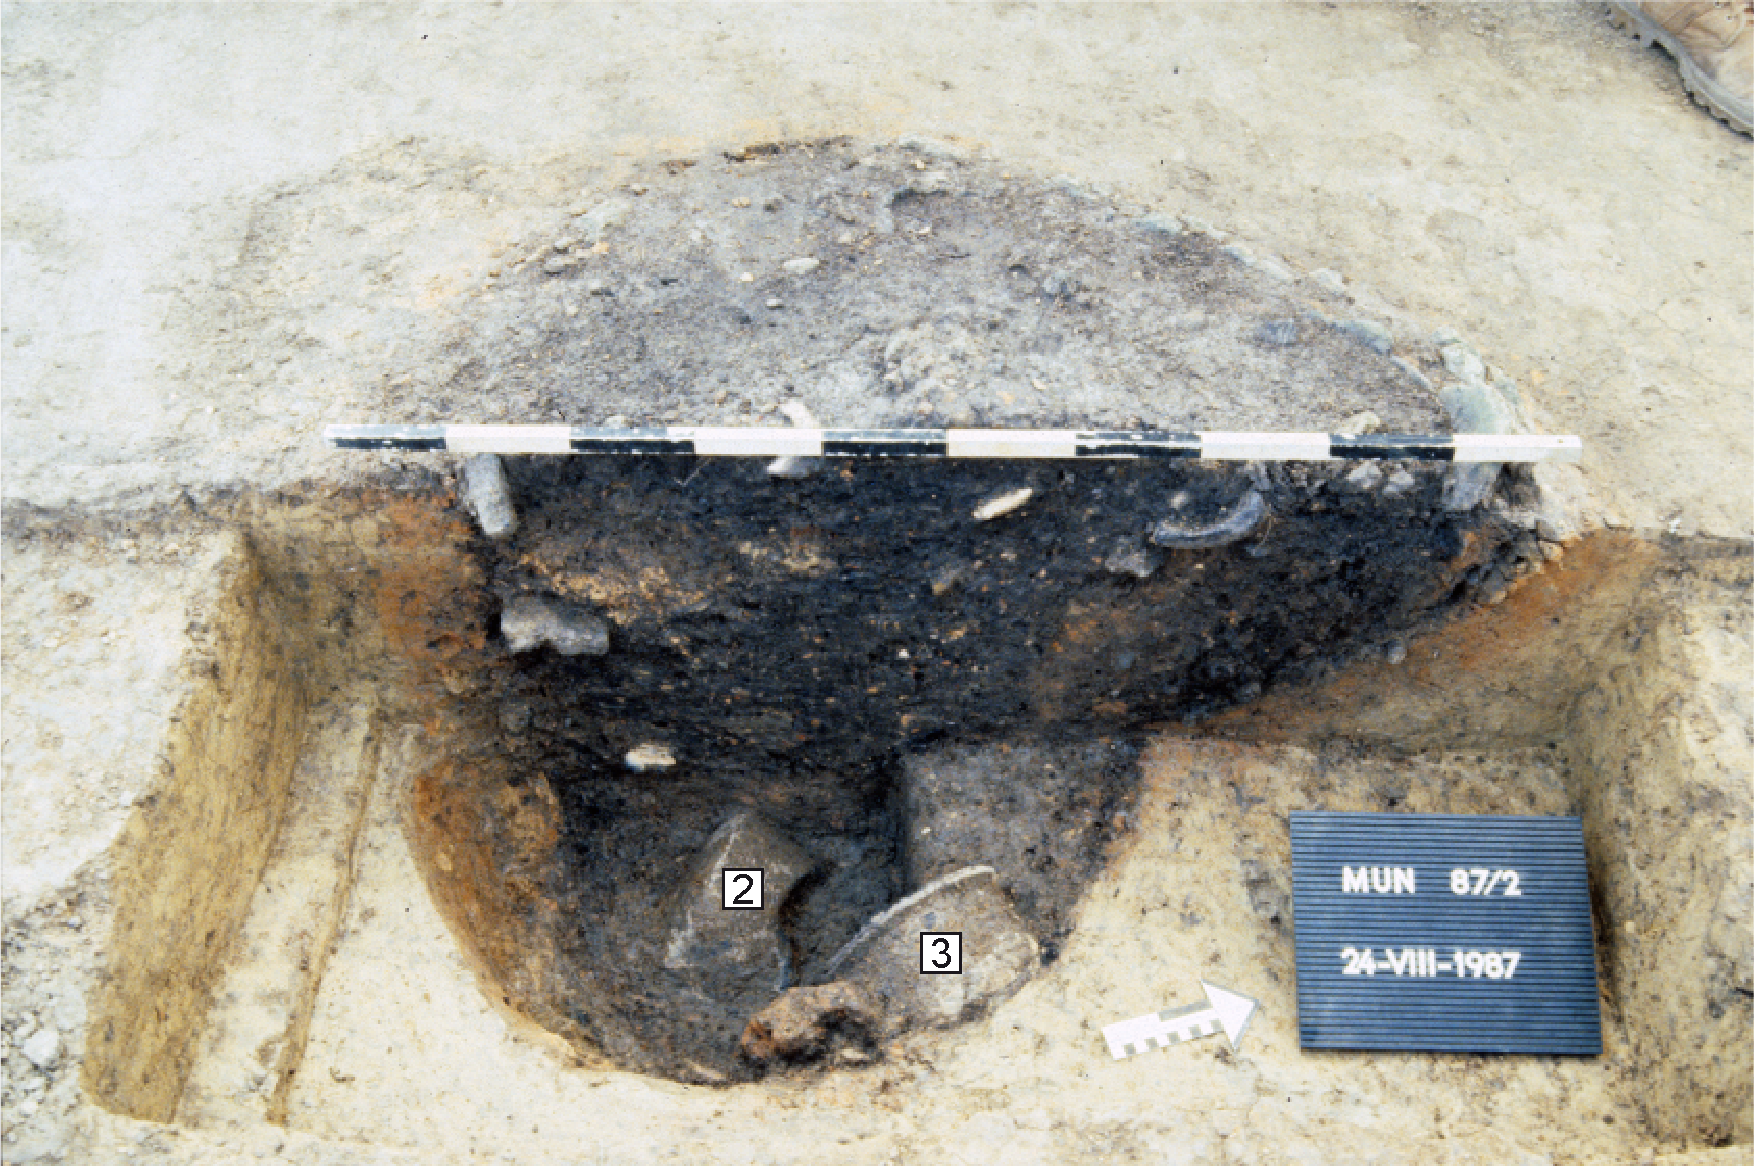
\includegraphics[width = \textwidth]{fig/MUN87-211-5_E87-041-26.pdf}
		\caption{Abtrag 5 (Foto: M. K. H. Eggert, 1987)}
		\label{fig:MUN87-211-5}
	\end{subfigure}\hfill
	\begin{subfigure}{\columnwidth}
		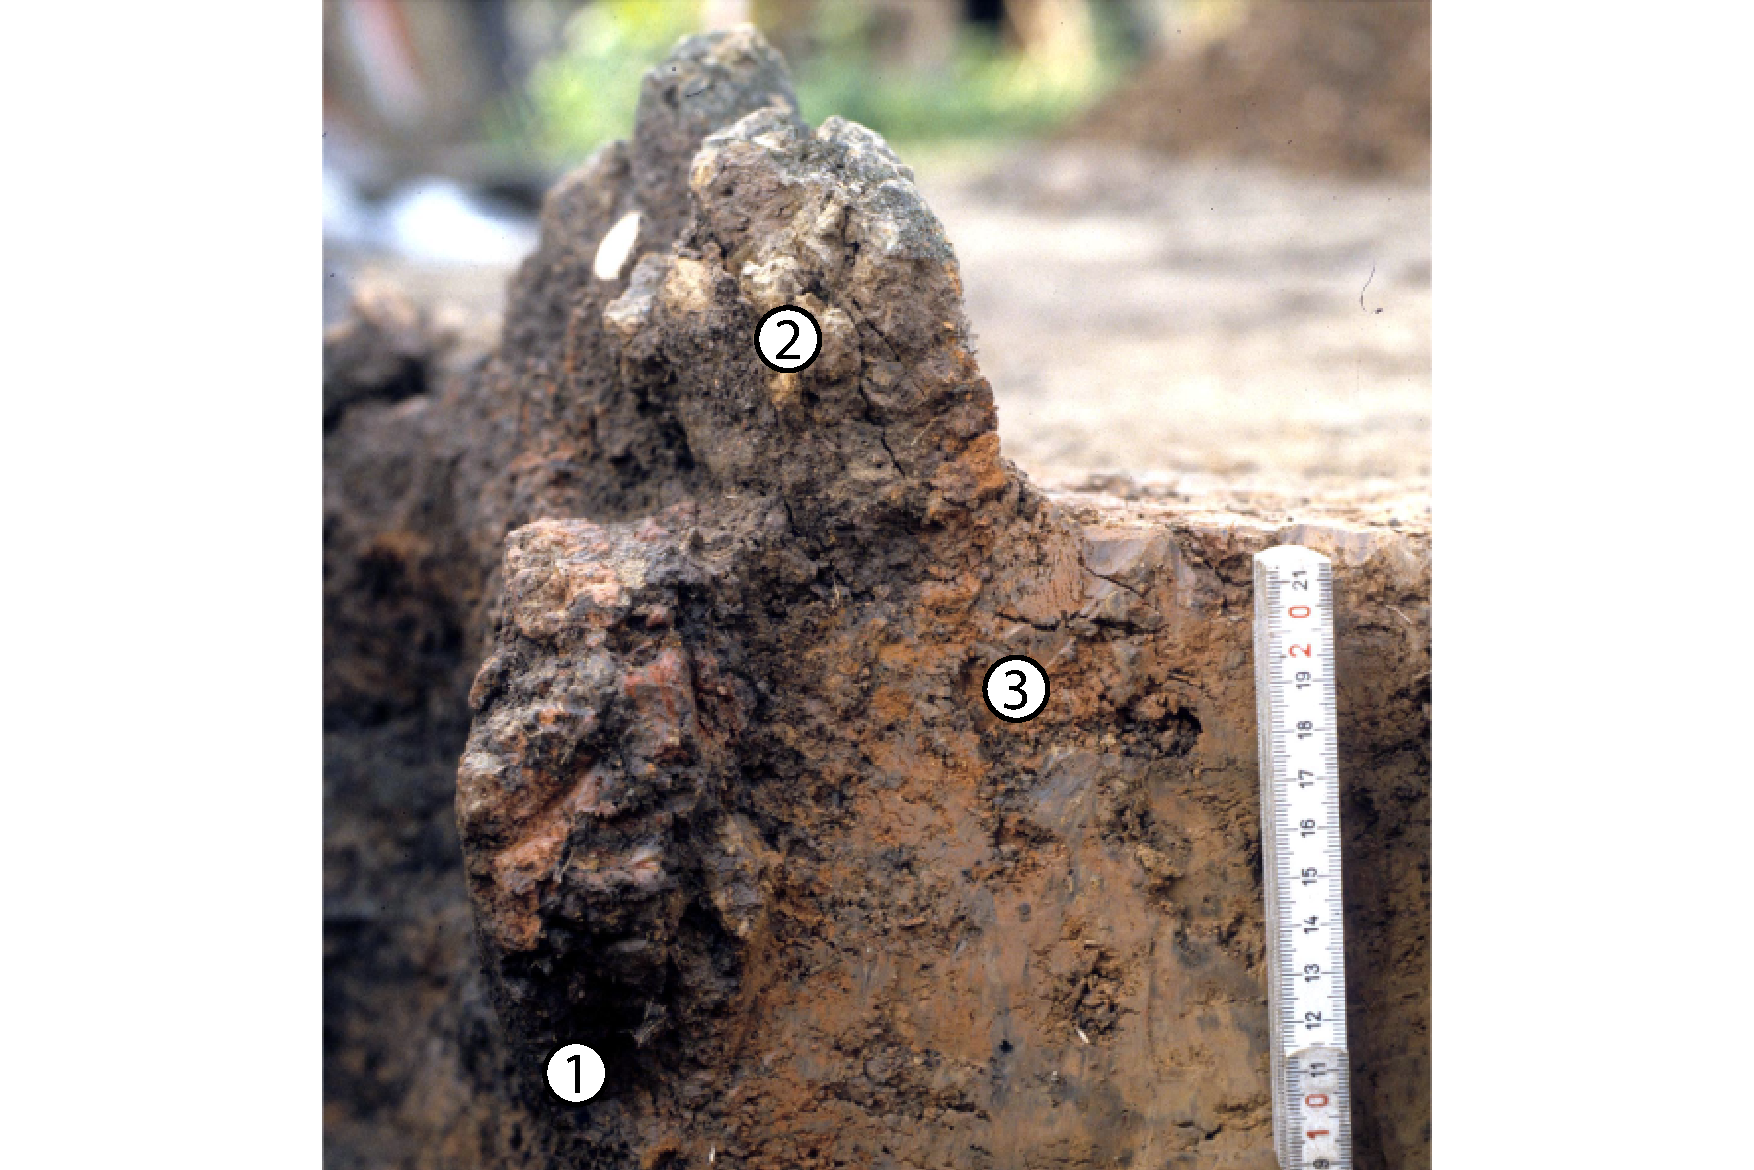
\includegraphics[width = \textwidth]{fig/MUN87-211-4_F87-02-31.pdf}
		\caption{Detail des Querprofils (West--Ost; Abb.~\ref{fig:MUN87-211-4_F87-02-36}; Foto: F. Nikulka, 1987).}
		\label{fig:MUN87-211-4_F87-02-31}
	\end{subfigure}
	\begin{subfigure}{\columnwidth}
		\centering
		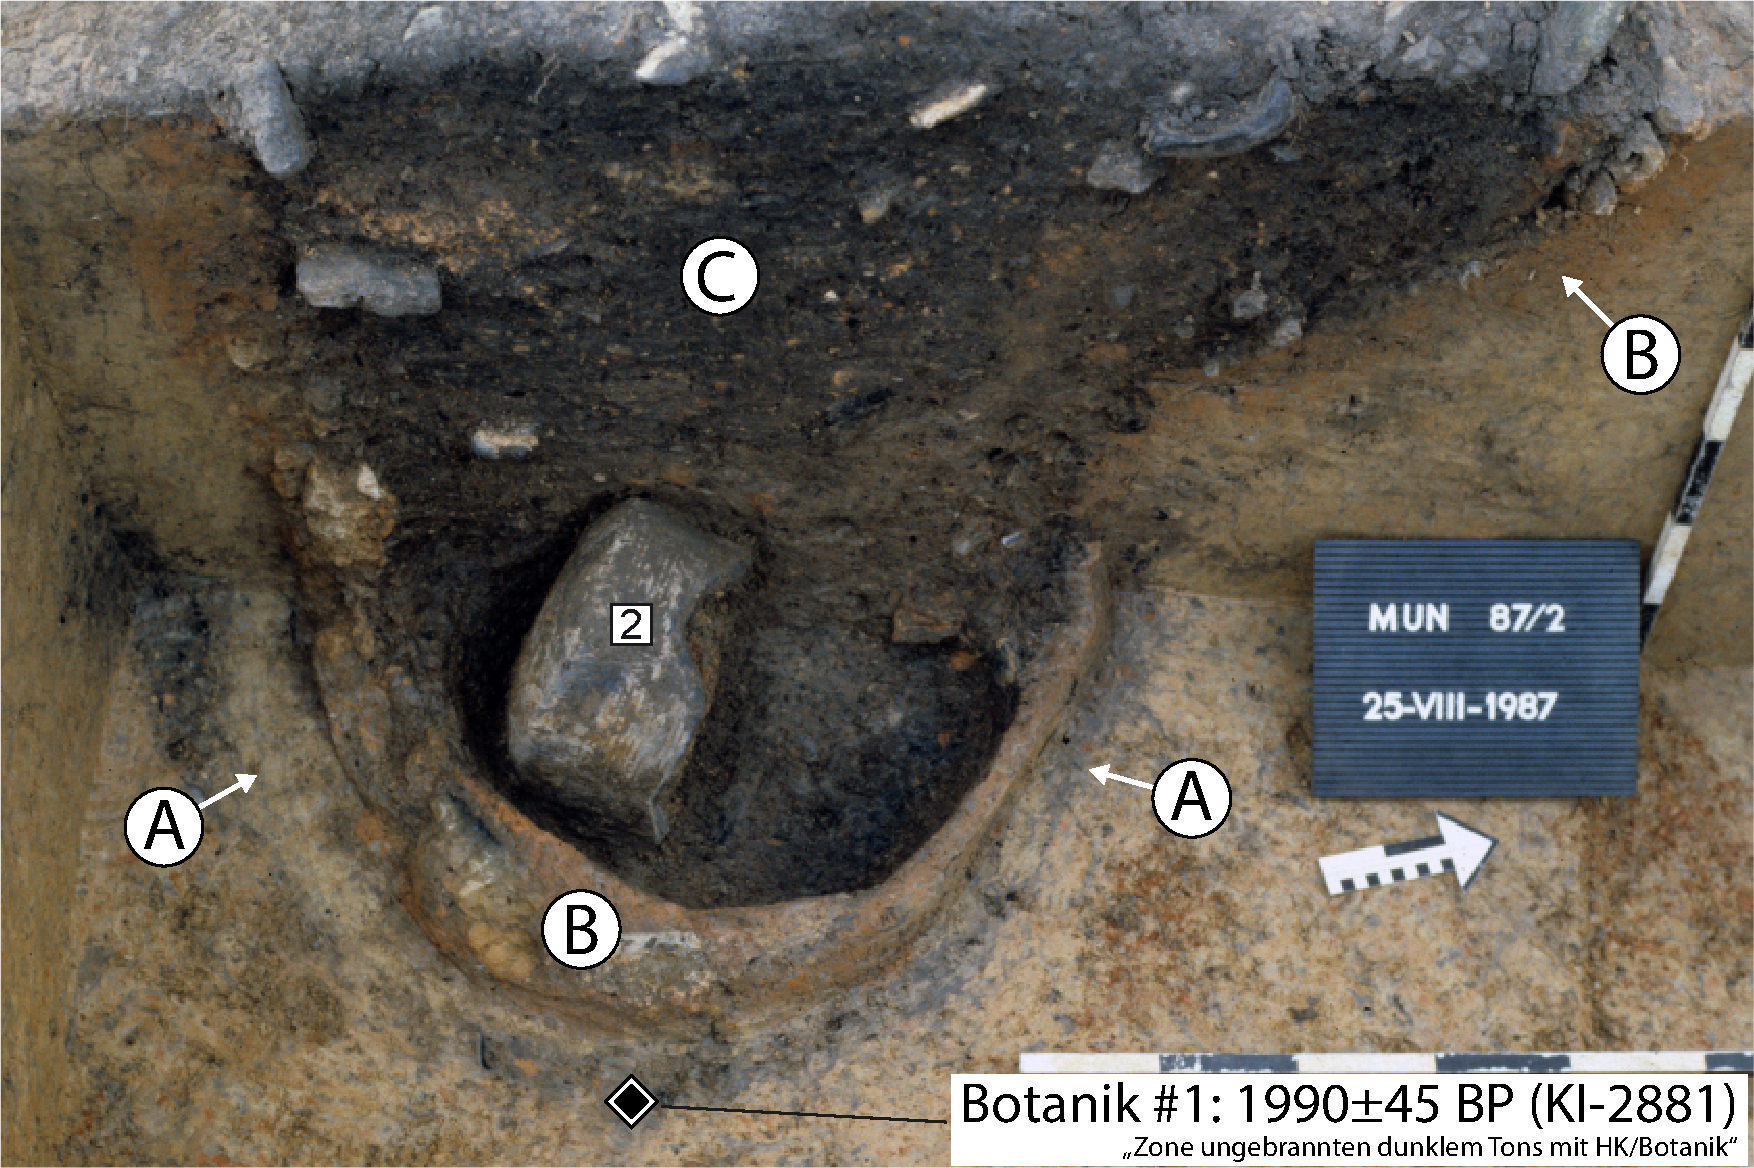
\includegraphics[width = \textwidth]{fig/MUN87-211-6_F87-03-16.pdf}
		\caption{Abtrag 6 (Foto: F. Nikulka, 1987)}
		\label{fig:MUN87-211-6}
	\end{subfigure}\hfill
	\begin{subfigure}{\columnwidth}
		\centering
		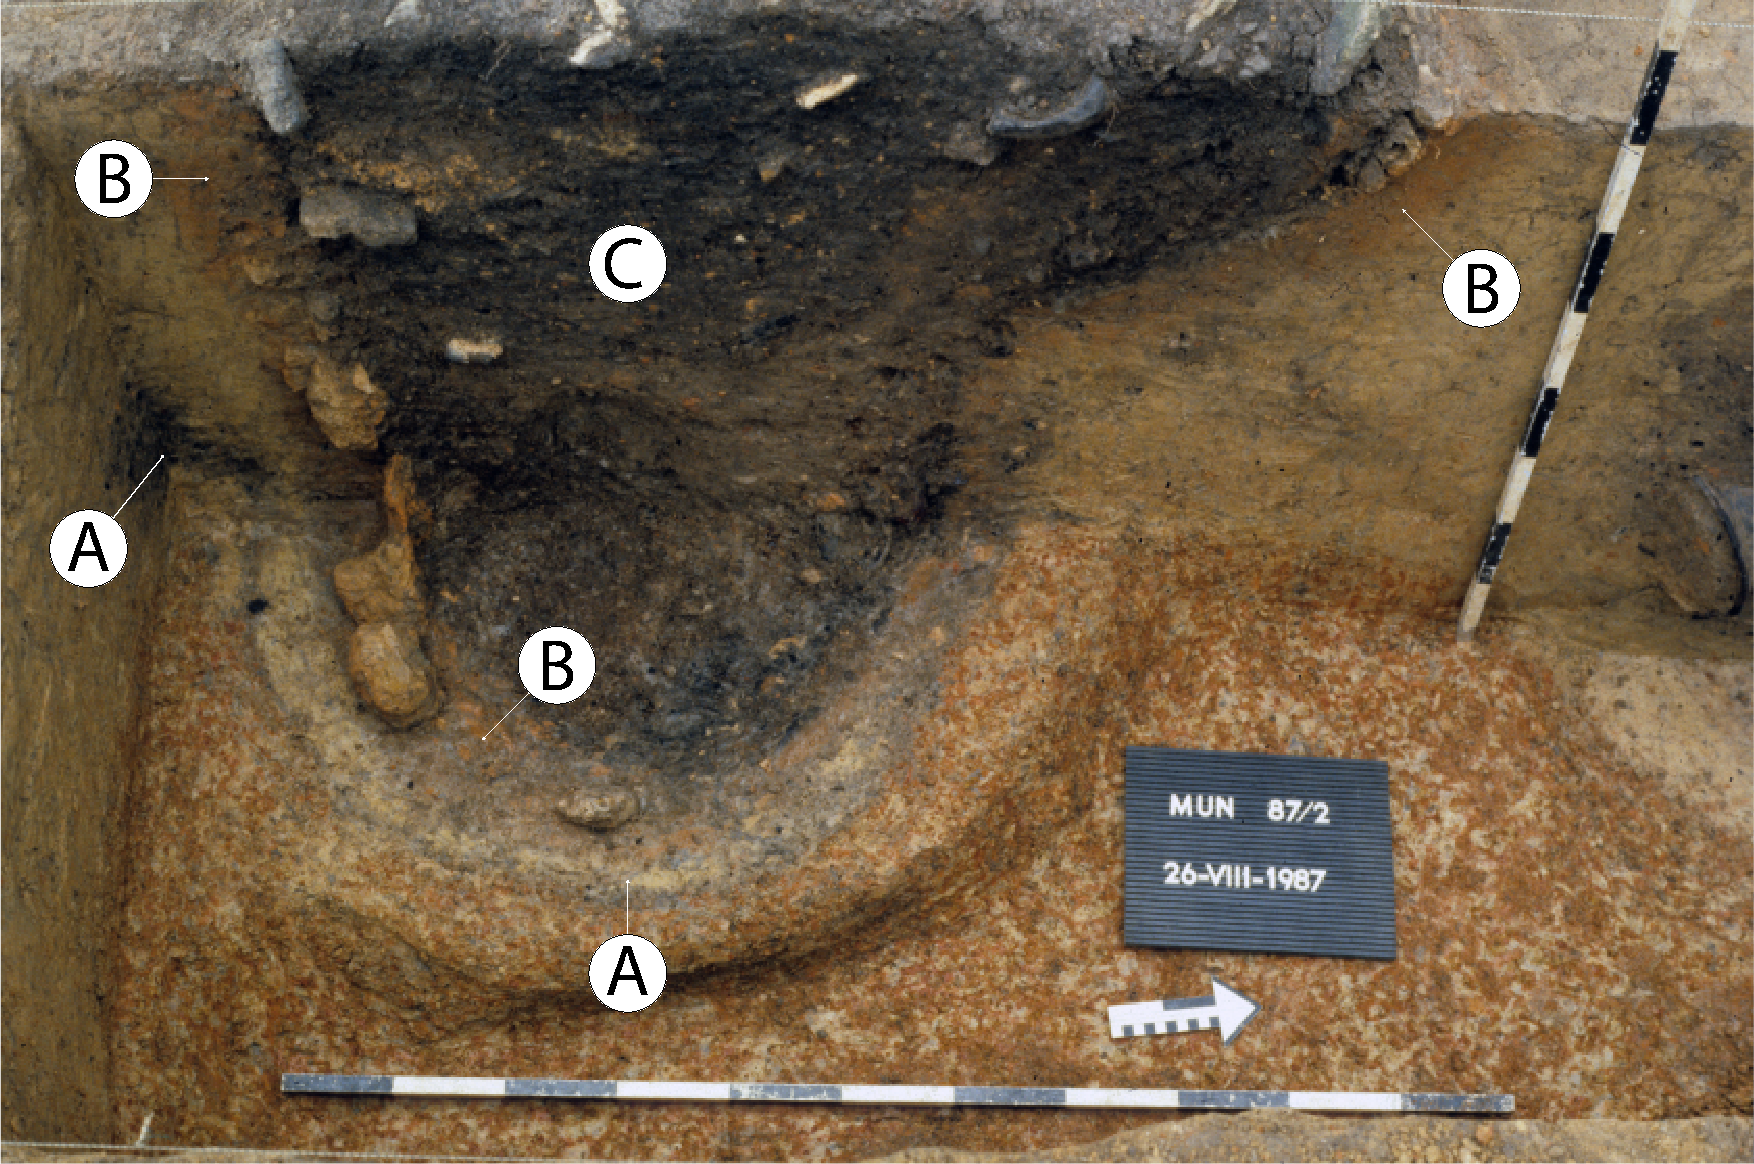
\includegraphics[width = \textwidth]{fig/MUN87-211-7_F87-03-26.pdf}
		\caption{Abtrag 7 (Foto: F. Nikulka, 1987)}
		\label{fig:MUN87-211-7.1}
	\end{subfigure}
	\begin{subfigure}{\columnwidth}
		\centering
		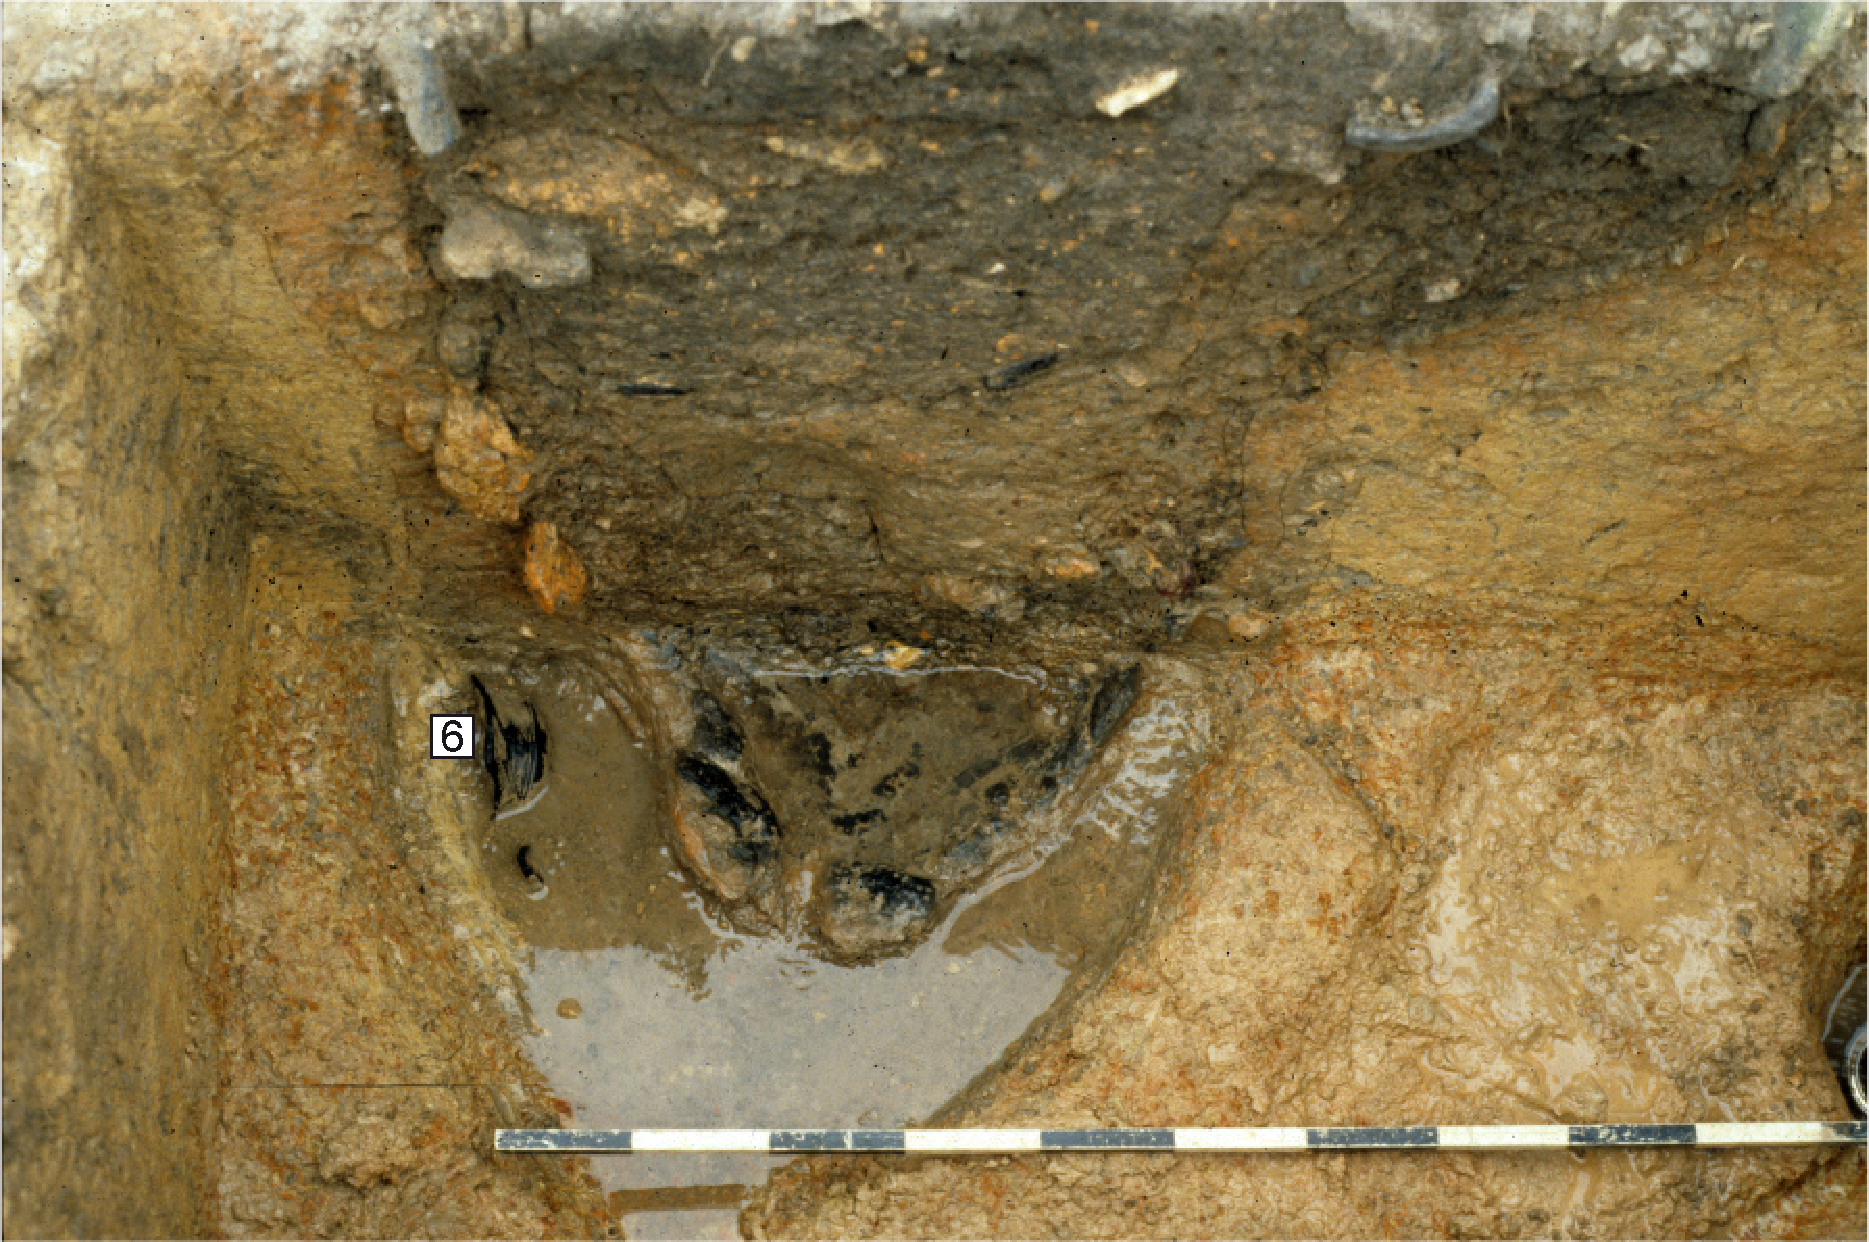
\includegraphics[width = \textwidth]{fig/MUN87-211-7_F87-03-36.pdf}
		\caption{unterhalb Abtrag 7 (Foto: F. Nikulka, 1987)}
		\label{fig:MUN87-211-7.2}
	\end{subfigure}\hfill
	\begin{subfigure}{\columnwidth}
		\centering
		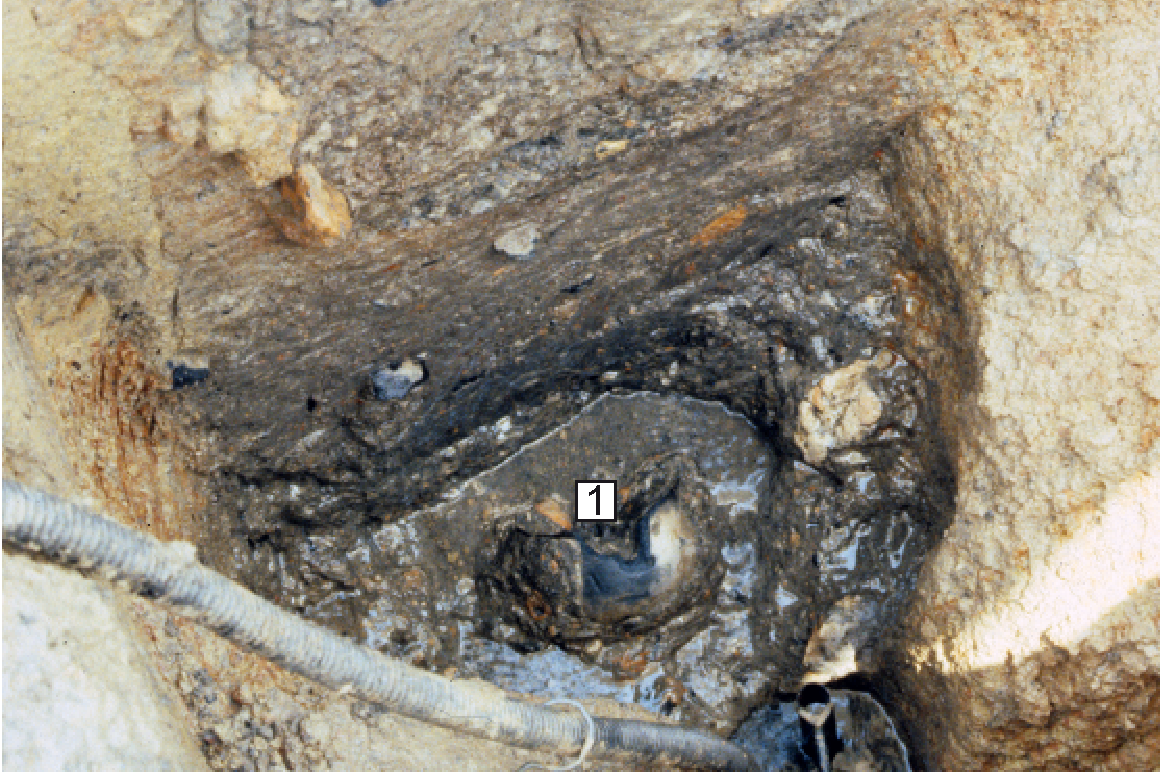
\includegraphics[width = \textwidth]{fig/MUN87-211-8_E87-046-2.pdf}
		\caption{Abtrag 8 (Foto: F. Nikulka, 1987)}
		\label{fig:MUN87-211-8}
	\end{subfigure}
	\caption{MUN~87/2-1-1: Abträge in der oberen (A--F) sowie unteren Verfüllung (G--H).}
	\label{fig:MUN87.2-1-1-5_Foto}\label{fig:MUN87-211_Oben}\label{fig:MUN87.2-1-1-7+8_Foto}
\end{figure*}

\begin{figure*}[p]
	\centering
	\includegraphics[width = \textwidth]{fig/MUN87-211.pdf}
	\caption{MUN~87/2-1-1: Planum und Profil.}
	\label{fig:MUN87.2-1-1_Planum+Profil_Zeichnung}
\end{figure*}

Im sechsten Abtrag wurde außerhalb der Lehmwanne B eine Zone ungebrannten Lehms mit verkohlten Palmkernen und Holzkohle beobachtet, die das oberen Ende des unteren Grubenteils A anzeigte (Abb.~\ref{fig:MUN87-211-6}--C). An der Sohle der Lehmwanne B fand sich eine deutliche Konzentration aus Schlacken (Abb.~\ref{fig:MUN87.2-1-1_Planum+Profil_Zeichnung}). Diese ließen sich leicht abheben und lagen auf einer zirka 1\,cm starken, durchgehenden Schicht aus rötlich-braunem, ungebannten Lehm auf.\footnote{Daraus schließt der Ausgräber, dass die Schlacke sekundär umgelagert wurde und zusammen mit der Keramik in der Grube deponiert wurde.}

Nach dem Abtrag der Lehmwanne B wurde die untere Grubenverfüllung A vollständig im Planum erfasst. In dieser bis etwa 1,5\,m unter die rezente Oberfläche reichenden Eingrabung fand sich ein zweites, intentionell deponiertes Inventar aus Keramikgefäßen, gebrannte Lehmbrocken oder Schlacken fanden sich in diesem Bereich hingegen nicht.\footnote{Bereits das Abtragen der Sohle der Lehmwanne B und der unteren Abschnitte der Verfüllung C wurde durch starke Regenfälle beeinträchtigt (Abb.~\ref{fig:MUN87.2-1-1-7+8_Foto}). Kontinuierliche Wassereinbrüche durch aus den Profilen nachlaufendes Regenwasser erschwerten die Grabung und Dokumentation. Die Grabung erfolgte in diesem Bereich auch nicht mehr auf der gesamten Breite des Schnittes.} Die Verfüllung des unteren Grubenbereichs A besteht aus homogenem dunkelgrauen und tonigem Material. Es enthielt größere Mengen botanischer Reste wie Fruchtschalen. In den untersten 0,2\,m verjüngte sich die Grube deutlich, während die Lateritisierung im anstehenden Lehm stärker wurde.

Die Grenzen der ursprünglich ausgehobenen Grube ließen sich im nördlichen Bereich durch die Lateritisierung gut bestimmen. Entlang seiner südlichen Grenze zog die Verfüllung jedoch noch in das Südprofil (Abb.~\ref{fig:MUN87.2-1-1_Planum+Profil_Zeichnung}). Es ist nicht nur möglich, sondern auch wahrscheinlich, dass die südliche Grenze der ursprünglich ausgehobenen Grube außerhalb des durch den Schnittkasten erfassten Bereiches lag (Abb.~\ref{fig:MUN87-211-6}, \ref{fig:MUN87.2-1-1_Planum+Profil_Zeichnung}: Schicht~9).

\begin{figure*}[tb]
	\centering
	\includegraphics[width=\textwidth]{fig/9-13_MUN87-211_Fragmentierung_2.pdf}
	\caption{MUN~87/2-1-1: Fragmentierungsgrad der Scherben (n~=~79; Größenklassen siehe Anm.~\ref{ftn:Keramik_Fragmentierung}).}
	\label{fig:MUN87-211_Fragmentierung}
\end{figure*}

\begin{table*}[tb]
	\centering{\footnotesize \begin{sftabular}{@{}lrrrr@{}}
\toprule
   \textbf{Fundkategorie} &  \textbf{Anzahl} &    \textbf{\%} &  \textbf{Gewicht (kg)} &    \textbf{\%} \\
\midrule
           Eisen &       1 &   0,1 &          0,03 &   0,1 \\
 gebrannter Lehm &      88 &  13,1 &          2,04 &   5,8 \\
         Keramik &      79 &  11,7 &          7,05 &  20,0 \\
          Metall &       1 &   0,1 &             - &     - \\
        Ofenwand &       - &     - &         18,24 &  51,8 \\
        Schlacke &     489 &  72,7 &          7,58 &  21,5 \\
          Sonder &       1 &   0,1 &          0,06 &   0,2 \\
          Tuyere &      14 &   2,1 &          0,22 &   0,6 \\
\bottomrule
\end{sftabular}
}
	\caption{MUN~87/1-2-1: Anteil verschiedener Fundmaterialien.}
	\label{tab:MUN87-2-1-1_Funde}
\end{table*}

\begin{figure*}[p]
	\centering
	\begin{subfigure}{\textwidth}	
		\centering
		\includegraphics[width = \textwidth]{fig/9-16_MUN87-211_VerteilungFunde_R.pdf}
		\caption{Fundmaterial.\vspace{1em}}	
		\label{fig:MUN87-211_VerteilungFunde}
	\end{subfigure}
	\begin{subfigure}{\textwidth}
		\centering
		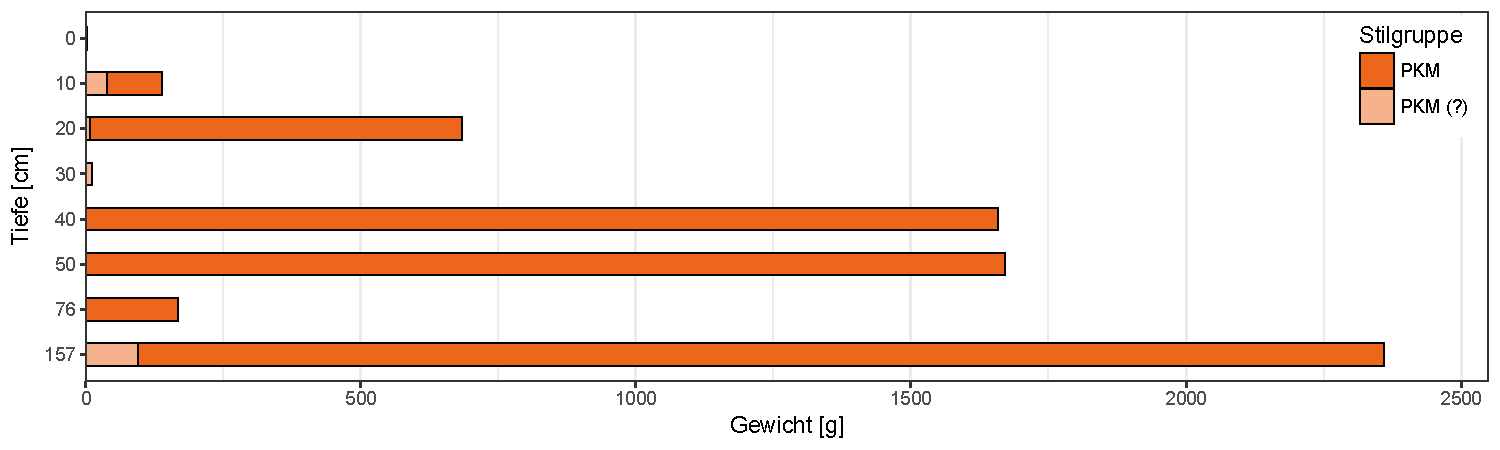
\includegraphics[width = \textwidth]{fig/9-16_MUN87-211_KeramikStilgruppen_R.pdf}
		\caption{Keramische Stilgruppen.\vspace{1em}}
		\label{fig:MUN87-211_VerteilungStilgr}
	\end{subfigure}
	\begin{subfigure}{\textwidth}	
		\centering
		\includegraphics[width = \textwidth]{fig/9-16_MUN87-211_Fabrics_R.pdf}
		\caption{\textit{Fabrics}.\vspace{1em}}
		\label{fig:MUN87-211_VerteilungFabrics}
	\end{subfigure}
	\begin{subfigure}{\textwidth}	
		\centering
		\includegraphics[width = \textwidth]{fig/9-16_MUN87-211_Schlacken_R.pdf}
		\caption{\textit{Schlacken}.}
		\label{fig:MUN87-211_Schlacken}
	\end{subfigure}
	\caption{MUN~87/2-1-1: Verteilung der Fundmaterialien (A), keramischen Stilgruppen (B), \textit{Fabrics} (C) und Schlacken (D) in den entsprechenden Tiefen der Grabung.}
	\label{fig:MUN87-211_Funde}
\end{figure*}

\vspace{1.5em}
\noindent Die Grabung erbrachte den folgenden stratigrafischen Befund (Abb.~\ref{fig:MUN87.2-1-1_Planum+Profil_Zeichnung}):\footnote{Das Gesamtprofil wurde nicht in einem Arbeitsgang dokumentiert. Aufgrund starker Regenfälle wurde das bis etwa zur Unterkante der Lehmwanne (B) freigelegte Profil gezeichnet. Der Verlauf der unteren Verfüllung (A) wurde später ergänzt.}
\begin{itemize}[leftmargin=*, labelindent=1.25em, noitemsep, topsep=0pt]
\item [C] Obere Verfüllung
\item [(1)] 10YR 3/1; stark humoser, leicht sandiger Lehm; Schlacke unterschiedlicher Art und Größe ungleichmäßig verteilt, vereinzelt Holzkohlepartikel (\O~0,5--1,0\,cm), vereinzelt verkohlte Fruchtschalenfragmente, wenige Partikel rotgebrannten Lehms (\O~bis 1,5\,cm), Keramik, Schlacke, Schachtfragmente
\item [(2)] 10YR 3/2; humoser Lehm, stark inhomogene Verteilung von Brocken und Partikeln von rot- und gelbgebranntem Lehm, Schlacke, sehr wenig Lateritpartikel
\item [(4)] 5YR 2.5/2; humoser Lehm, stark durchmischt mit unterschiedlich großen (\O~1--3\,cm) Partikeln rotgebrannten Lehms, Holzkohle, Keramikscherben, Schlacke
\item [(5)] 5YR 4/4; rötlich-brauner Lehm, durchmischt mit rotgebranntem Lehm, Schlacke
\item [(6)] 10YR 3/3; dunkelbrauner Lehm, Keramik, vereinzelt Holzkohle, keine Schlacke
\item [(7)] 10YR 3/3; starke Schlackeanreicherung, durchmischt mit Lehm, keine Holzkohle, ein Keramikstück, Schlackenstücke unterschiedlicher Größe
\item [(8)] 7.5YR 3/4; sehr starke Schlackeanreicherung, mit zunehmender Tiefe dichter und fester werdend, Holzkohle, ein Lateritbrocken
\item [(9)] 10YR 4/4; ungebrannter dunkler Ton, Holzkohle, relativ viele Fragmente von Fruchtschalen (verkohlt), Einschlüsse von ungebranntem gelben Lehm
\item [B] Lehmwanne
\item [(3)] 2,5YR 5/8 (red); rotgebrannter Lehm mit Einschlüssen aus verziegelten Lehmbrocken
\item [A] Untere Verfüllung
\item [(12)] 10YR 3/3 (dark brown); dunkelgrauer Ton
\item [(13)] 10YR 3/2 (very dark grayish brown); schwarz-grauer Ton
\end{itemize}

\newpage\paragraph{Keramik\vspace{.5em}}\mbox{}\\
\begin{tabular}{@{}lrl@{}}
Ausgezählt: & 359\,g & \\ 
Bearbeitet: & 6692\,g & (95\,\%) \\ 
Insgesamt: & 7051\,g & \\ 
\end{tabular} 

\vspace{1em}
\noindent Beiden Verfüllungsbereiche (A und C) enthalten jeweils stilistisch homogene Inventare des Pikunda-Munda-Stils (Kap.~\ref{sec:PKM-Gr}). Das Inventar der oberen, stratigrafisch jüngeren Verfüllung (C) besteht fast vollständig aus Gefäßen und großen Gefäßteilen, die auf der Seite oder Mündung liegend deponiert wurden (Abb.~\ref{fig:MUN87-211-3_F87-02-27}--E). Im stratigrafisch älteren, unteren Grubenteil (A) sind die Gefäße ebenfalls auf der Seite oder Mündung liegend deponiert worden.\footnote{Gefäß 1 (Abb.~\ref{fig:MUN87-211-8}) weist schwarze, organische  Anhaftungen am Gefäßboden auf. Vier Schalen des Typs E3 zeigen einen auffällig weiß-oxidierten Gefäßboden. Die Außenseiten der Gefäße sind stark \textit{fleckig}, während die Innenseiten in der Regel gleichmäßig gefärbt sind. Zudem fanden sich in der unteren Verfüllung (A) neben den Gefäßen und großen Gefäßfragmenten auch einige kleine Einzelscherben (24\,\%). Nicht den Gefäßen zuordenbare Einzelscherben sind im oberen Verfüllungsbereich (C) hingegen eine klare Ausnahme (4\,\%).}

Bezüglich der stilistischen Charakteristika ergeben sich zwischen den Inventaren aus den beiden Verfüllungen einige Unterschiede (siehe Kap.~\ref{sec:PKM-Gr}). Der obere Grubenteil (C) enthält ein keramisches Inventar, welches durch Pikunda-Munda-Schalen des Typs F3 bestimmt wird (Taf.~91.1--5). Diese heben sich mit ihrem scharfen Profilknick zwischen einem geraden, bis leicht konkavem Gefäßbauch und einem runden Boden deutlich von den Schalen des Typs E3 aus dem unteren Inventar (A) ab. Die Verzierungen der Gefäße des oberen Bereichs beschränken sich fast ausschließlich auf die Gefäßbäuche. Die Gefäße sind regelhaft mit horizontalen, vertikalen oder bogenförmigen, etwa 3--4\,mm breiten Rillen verziert (Tab.~\ref{tab:Verzierungselemente}: 02.1). Die Rillen überlagern häufig ein flächiges Wiegebandmuster (04.2). Selten wurden auch einzelne Rillen an der Innenseite der Ränder beobachtet.\footnote{Gerillte Mündungen, die bei den Schalen des Typs F3 aus der oberen Verfüllung (C) beobachtet werden konnten, fanden sich an keiner GE aus dem unteren Bereich (A). Die hier gefundenen Schalen weisen schräg nach außen abgestrichene oder runde Randlippen auf. In beiden Inventaren machen konkav ausbiegende Ränder vom Typ B2 jeweils etwa die Hälfte der Formen aus. Gerade ausbiegende Ränder des Typs B1, wie sie im oberen Grubenteil (C) zu etwa 20\,\% vorkommen, finden sich im unteren Inventar des Bereichs A nicht.}

Im unteren Grubenteil (A) finden sich keine Schalen mit scharfem Bauchknick des Typs F3. Die Gefäße aus diesem Bereich sind durchweg Schalen des Typs E3 mit einem runden, konvexem Umbruch zwischen dem konkavem Bauch und dem Bodenansatz. Die Ränder und Gefäßbäuche sind mit feineren Rillenmustern verziert, als die Keramik aus dem oberen Bereich (C). Die Verzierungen bestehen vor allem aus horizontalen Bändern aus 1--2\,mm breiten, feinen Rillen und Winkelmustern. Wiegebandverzierung wurde an keiner GE aus der unteren Verfüllung (A) beobachtet. Das Inventar entspricht mit Blick auf die Gefäßformen und Verzierungen nahezu exakt den GE aus der direkt benachbarten Grube MUN~87/2-1-3 (Kat.-Nr.~17).

In beiden Inventaren sind, anders als etwa bei der Pikunda-Munda-Keramik aus Pikunda am \mbox{Sangha} (Fpl.~255; Kat.-Nr.~8), die Gefäßböden unverziert. Die Grabung MUN~87/2-1-1 ist der einzige Befund, der eine stratigrafische wie auch eine stilistische Differenzierung der Pikunda-Munda-Keramik erkennen lässt.

\begin{figure*}[p]
	\begin{minipage}[b]{.66\textwidth}
		\includegraphics[width = \textwidth]{fig/MUN87-211-2_Eisengeld.jpg}
	\end{minipage}\hfill
	\begin{minipage}[b]{.3\textwidth}
		\caption{~87/2-1-1: Eisenobjekt (Fotos links: D. Seidensticker, 2012; rechts: R. Müller/RGZM, 2012).}\label{fig:MUN87.2-1-1-2_Eisengeld_Foto}
	\end{minipage}
\end{figure*}

\begin{table*}[p]
	\centering{\footnotesize
		\begin{sftabular}{@{}llllll@{}}
			\toprule
			\textbf{Lab-Nr} & \textbf{Datum (bp)} & \textbf{Datum (2-Sigma)} & \textbf{Bereich} & \textbf{Abtrag} & \textbf{\begin{tabular}[t]{@{}l@{}}Tiefe\\ (unter NP)\end{tabular}} \\ 
			\midrule
			KI-2881 & 1990\( \pm \)45 & \begin{tabular}[t]{@{}l@{}}107 v.~Chr.--90 n.~Chr. (92,7\,\%)\\ 99--124 n.~Chr. (2,7\,\%)\end{tabular} & A & 6 (Botanik 1) & 0,93\,m \\ 
			KI-2885 & 1800\( \pm \)80 & 55--401 n.~Chr. & C & 4 (HK 6) & 0,62\,m \\ 
			KI-2886 & 1910\( \pm \)80 & \begin{tabular}[t]{@{}l@{}}94 v.~Chr.--260 n.~Chr. (92,3\,\%)\\ 279--326 n.~Chr. (3,1\,\%)\end{tabular} & A & 6 (HK 8) & 0,98\,m \\ 
			KI-2887 & 2020\( \pm \)180 & \begin{tabular}[t]{@{}l@{}}476--444 v.~Chr. (0,6\,\%)\\ 431 v.~Chr.--405 n.~Chr. (94,8\,\%)\end{tabular} & C & 7 (HK 9) & 1,02\,m \\ 
			\bottomrule 
	\end{sftabular}}
	\caption{MUN~87/2-1-1: Radiokohlenstoffdatierungen.}
	\label{tab:MUN87-211_14C-Daten}
\end{table*}

\begin{figure*}[p]
	\centering
	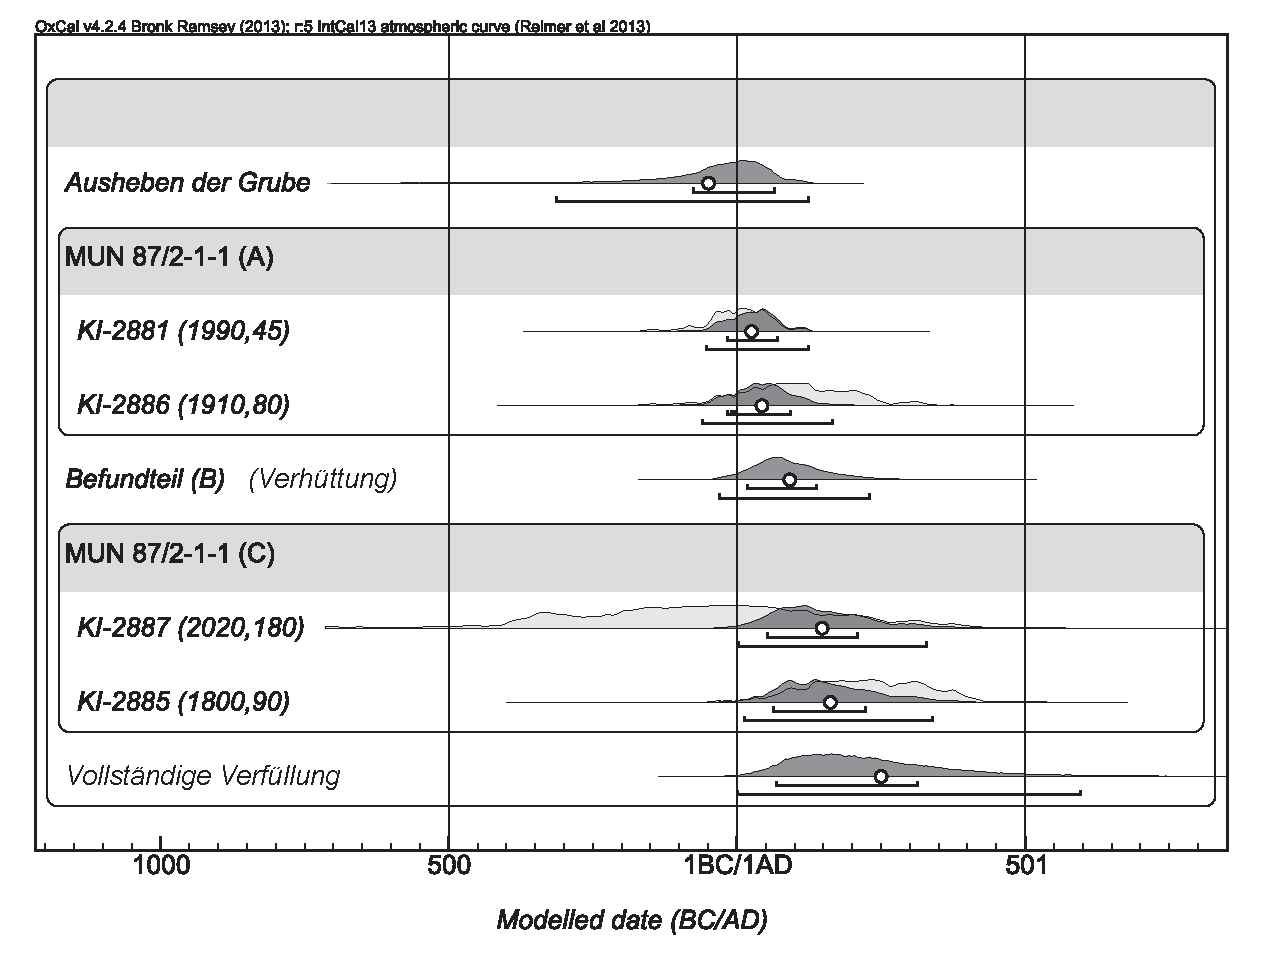
\includegraphics[width = .75\textwidth]{fig/MUN87_2_1_1_14C.pdf}
	\caption{MUN~87/2-1-1: Datierung der Phasen des Befundes auf Basis der Radiokohlenstoffdatierungen.}
	\label{fig:MUN87-2-1-1_14C_OxCal}
\end{figure*}

\paragraph{Sonstige Funde}\hspace{-.5em}|\hspace{.5em}%
Das Fundmaterial umfasst -- neben der Keramik -- auch fast 20\,kg gebrannten Lehm; die Reste der Ofenwanne (B; Abb.~\ref{fig:MUN87-211_VerteilungFunde}; Tab.~\ref{tab:MUN87-2-1-1_Funde}). Die Fragmente sind bis zu 15\,cm groß und hellgelb bis leicht rötlich gefärbt. Einige Stücke weisen auf einer Seite eine schwarze Reduktionszone auf.\footnote{Siehe Abb.~\ref{fig:MUN87-1_Ofenwand}.} Die Lehmmatrix enthält, neben einer Vielzahl nicht genauer identifizierbarer, nichtplastischer Materialien, auch bis zu 5--8\,mm große, teilweise stark verrundete Lateritstücke. Abdrücke von Stangen oder ähnlichem finden sich selten. Die wenigen beobachteten Stangenabdrücke haben einen Durchmesser von 5--6\,cm.

Die insgesamt knapp 7\,kg Schlacke stammen sämtlich aus dem oberen Befundteil (C). Die Schlacke wurde nach dem Ausräumen des Verhüttungsbefundes zusammen mit den Gefäßen in der Grube deponiert. Es dominieren kantige Verhüttungsschlacke geringer Viskosität (Typ 4a und 4b; Abb.~\ref{fig:MUN87-211_Schlacken}). Anders als im Befund MUN~87/1 (Kat.-Nr.~15) sind nur wenige Stücke grünlich gefärbt. In etwa zu gleichen Teilen fanden sich bläuliche und grünliche Fließschlacke hoher Viskosität (Typ 2a und 2b).

\begin{figure*}[!tb]
	\centering
	\begin{subfigure}[t]{0.32\textwidth}
		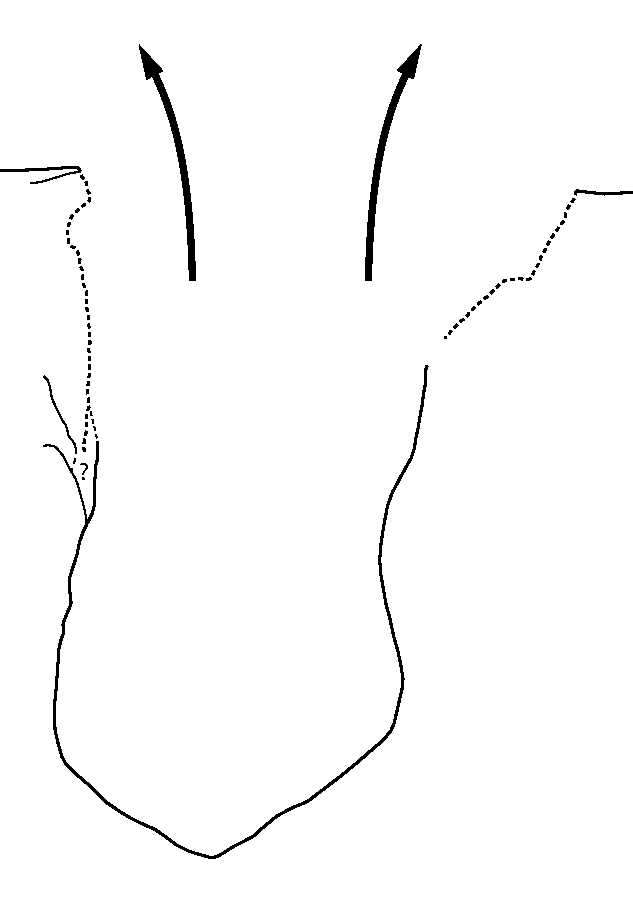
\includegraphics[width = \textwidth, page = 1]{fig/MUN87-211_Ablauf.pdf}
		\caption{Ausheben der Grube.}
		\label{fig:MUN87.2-1-1_Sequenz_Skizze_01}
	\end{subfigure}\hspace{2mm}
	\begin{subfigure}[t]{0.32\textwidth}
		\includegraphics[width = \textwidth, page = 2]{fig/MUN87-211_Ablauf.pdf}
		\caption{\textbf{A}: Deponierung des Inventars A und Verfüllen der Grube; unklar, ob bis zur Geländeoberkante oder nur teilweise.}
		\label{fig:MUN87.2-1-1_Sequenz_Skizze_02}
	\end{subfigure}\hspace{2mm}
	\begin{subfigure}[t]{0.32\textwidth}
		\includegraphics[width = \textwidth, page = 3]{fig/MUN87-211_Ablauf.pdf}
		\caption{Anlage des Ofens -- Lehmauskleidung; unklar, ob in einer nur teilweise verfüllten Grube oder ob sie wieder ausgehoben wurde.}
		\label{fig:MUN87.2-1-1_Sequenz_Skizze_03}
	\end{subfigure}
	\begin{subfigure}[t]{0.32\textwidth}
		\includegraphics[width = \textwidth, page = 4]{fig/MUN87-211_Ablauf.pdf}
		\caption{\textbf{B}: Nutzung als Verhüttungsplatz und Verziegelung der Grubenwandung.}
		\label{fig:MUN87.2-1-1_Sequenz_Skizze_04}
	\end{subfigure}\hspace{2mm}
	\begin{subfigure}[t]{0.32\textwidth}
		\includegraphics[width = \textwidth, page = 5]{fig/MUN87-211_Ablauf.pdf}
		\caption{Ausräumen der Verhüttungsprodukte, Schlacke und Teile der Wandung.}
		\label{fig:MUN87.2-1-1_Sequenz_Skizze_05}
	\end{subfigure}\hspace{2mm}
	\begin{subfigure}[t]{0.32\textwidth}
		\includegraphics[width = \textwidth, page = 6]{fig/MUN87-211_Ablauf.pdf}
		\caption{\textbf{C}: Deponierung von Schlacke sowie Inventar C und Verfüllung des Befundes.}
		\label{fig:MUN87.2-1-1_Sequenz_Skizze_06}
	\end{subfigure}
	\caption{MUN~87/2-1-1: Generalisierte Darstellung der rekonstruierten Befundgenese.}
	\label{fig:MUN87.2-1-1_Sequenz_Skizze}
\end{figure*}

Ein flaches Eisenobjekt wurde unterhalb einiger Gefäßfragmente, in der Mitte des oberen Bereichs (C) gefunden (Abb.~\ref{fig:MUN87.2-1-1_Planum+Profil_Zeichnung}).\footnote{2012 wurde das Stück im Römisch-Germanischen Zentralmuseum Mainz (RGZM) restauriert.} Das Stück ist noch 136\,mm lang und 42\,mm breit (Abb.~\ref{fig:MUN87.2-1-1-2_Eisengeld_Foto}). Das erhaltene Ende ist leicht rautenförmig und maximal 20\,mm breit. Es läuft in einem quadratisch ausgeformten Dorn aus. Die Dicke des Stückes schwankt zwischen nur 1\,mm in der Mitte bis zu 3\,mm im Bereich der Endplatte.\footnote{Formal erinnert das Objekt an in Zentralafrika weit verbreitete Formen von \textit{Eisengeld}, wie sie unter anderem in Gräbern in Campo, Südkamerun ausgegraben wurden \parencite[siehe][119 Abb.~6.17, 122, 138, 194.1--2, 208.1--2]{Eggert.2016}.}

\paragraph{Datierung}\hspace{-.5em}|\hspace{.5em}%
Aus dem Befund MUN~87/2-1-1 liegen insgesamt vier Radiokohlenstoffdatierungen vor (Abb.~\ref{fig:MUN87-2-1-1_14C_OxCal}; Tab.~\ref{tab:MUN87-211_14C-Daten}). Die Probennahmestellen sind auf Basis der vorliegen Dokumentation nicht mehr zweifelsfrei nachvollziehbar. Einzig die Entnahmestelle der aus der Botanikprobe 1 entnommene Datierungsprobe KI-2881 kann, basierend auf einer Handskizze sowie nivellierten Tiefe, genau beschrieben werden (Abb.~\ref{fig:MUN87-211-6}; \ref{fig:MUN87.2-1-1_Planum+Profil_Zeichnung}).\footnote{In der Handskizze des sechsten Abtrags wird diese Probe direkt an der östlichen Grenze des Befundes verortet, außerhalb der gebrannten Lehmwanne (B). In der schriftlichen Dokumentation wird dieser Bereich als \enquote{Zone ungebrannten dunklen Tons mit Holzkohle und Botanik} beschrieben.} Für die übrigen drei Datierungen sind neben den Tiefen keine genauen Angaben zu den Probennahmestellen bekannt. Die Datierungsprobe KI-2886 wurde laut der schriftlichen Dokumentation ebenfalls aus der \enquote{Zone ungebrannten dunklen Tons mit Holzkohle und Botanik} genommen; wie auch KI-2881. Die beiden Proben spiegeln das Alter des unteren Befundteils (A) wider. Die Holzkohleprobe für die Datierung KI-2887 lag \enquote{auf [der] Bodenwanne} auf. Sie lässt sich somit zweifelsfrei der stratigrafisch jüngeren Verfüllung (C) zurechnen. Einzig für die vierte Datierung KI-2885 liegen außer der Tiefe keinerlei Angaben vor. Die Probe wurde im Abtrag 5 entnommen, in dem sich der untere Befundteil (A) noch nicht abzeichnete. Die Datierung kann folglich mit dem oberen Befundteil (C) assoziiert werden.

Die beiden Befundteile, die Deponierung im oberen Befundteil (C), sowie die ursprüngliche Keramikdeponierung im unteren Bereich (A), sind durch jeweils zwei Proben datiert (Abb.~\ref{fig:MUN87-2-1-1_14C_OxCal}, Tab.~\ref{tab:MUN87-211_14C-Daten}). Die beiden Radiokohlenstoffdatierungen aus dem unteren Grubenteil (KI-2881, KI-2886) erbrachten ein nahezu identisches Alter und decken kalibiert das 1.~Jh. v.~Chr. bis 3.~Jh. n.~Chr. ab.\footnote{Diese Altersspanne deckt sich auffällig gut mit den beiden Datierungen für die benachbarte Keramikdeponierung in der Grube MUN~87/2-1-3 (Kat.-Nr.~17).} Im Gegensatz dazu streuen die beiden aus dem stratigrafisch jüngeren Befundteil (C) stammenden Datierungen (KI-2885, KI2887). Sie decken nach der Kalibration einen Zeitraum vom 5.~Jh. v.~Chr. bis 5.~Jh. n.~Chr. ab. Während die Datierung KI-2887 aufgrund ihres hohen Standardfehlers eine weite Alterspanne erzeugt, ist die zweite Datierung aus dem oberen Befundteil (KI-2885) leicht jünger als die beiden Proben aus der stratigrafisch älteren Verfüllung A. Eine eindeutige chronologische Differenzierung der beiden Grubenteile auf Basis der Radiokohlenstoffdatierungen ist jedoch nicht möglich, da sich alle Datierungen in der 2-Sigma-Kalibration überlagern.

\paragraph{Interpretation}\hspace{-.5em}|\hspace{.5em}%
Durch die Grabung MUN~87/2-1-1 wurde ein Befund ausgegraben, der eine eindeutige Mehrphasigkeit aufweist. Der unterer Bereich (A) ist durch eine Deponierung von Gefäßen des Pikunda-Munda-Stils in einer Grube gekennzeichnet (Abb.~\ref{fig:MUN87.2-1-1_Sequenz_Skizze_02}). Diese Deponierung weist erstaunlich starke Parallelen zum grob zeitgleichen Befund MUN~87/2-1-3 (Kat.-Nr.~17) auf. Wie weit die ursprüngliche Eingrabung verfüllt wurde, bevor ein Bereich bis etwa 0,8--0,9\,m unter der heutigen Oberfläche mit Lehm ausgekleidet wurde (Abb.~\ref{fig:MUN87.2-1-1_Sequenz_Skizze_03}), lässt sich nicht mehr nachvollziehen. Die mit Lehm ausgekleidete Grube wurde für mindestens einen Verhüttungsprozess genutzt, wodurch die Lehmauskleidung verziegelt ist (Abb.~\ref{fig:MUN87.2-1-1_Sequenz_Skizze_04}). Nach dieser Nutzung wurde der Verhüttungsraum ausgeleert, vermutlich um an die Verhüttungsprodukte zu gelangen (Abb.~\ref{fig:MUN87.2-1-1_Sequenz_Skizze_05}). Im Anschluss wurde der Befund mit einer zweiten Deponierung von Gefäßen sowie Schlacke verfüllt (Abb.~\ref{fig:MUN87.2-1-1_Sequenz_Skizze_06}).

Die ursprüngliche Grube A war mindestens 1,55\,m tief und hatte einen Durchmesser von zirka 0,8\,m, wobei jedoch möglicherweise nicht die komplette Ausdehnung des ursprünglichen Befundes erfasst wurde. Der später in die Verfüllung der Grube A integrierte Verhüttungsbefund B reichte bis 0,8--0,9\,m unter die heutige Oberfläche und hatte dort einen Durchmesser von etwa 1,1\,m. Unterhalb von etwa 0,35\,m verjüngt sich die Lehmwanne und endet in einer nahezu runden Bodenwanne mit einem Druchmesser von 0,8\,m. Das Fehlen von sekundären Brandspuren an der Keramik und das einfache Ablösen der Schlacken legen nahe, dass die Lehmwanne im Anschluss an mindestens einen Verhüttungsprozess ausgeleert wurde. Wie viel Zeit zwischen der Deponierung in der ursprünglichen Grube A und der Anlage des Verhüttungsbefundes B vergangen war, lässt sich nicht mehr bestimmen. Da sich die Radiokohlenstoffdatierungen aus den beiden Bereichen in der 2-Sigma-Kalibation überlagern, kann auch der leichte stilistische Wandel der beiden Keramikinventare nicht zweifelsfrei chronologisch gedeutet werden.